\documentclass[article, a4paper]{llncs}

\usepackage{ucs} 
\usepackage[utf8x]{inputenc} % Включаем поддержку UTF8  
\usepackage[russian]{babel}  % Включаем пакет для поддержки русского языка  
\usepackage{csquotes}
\usepackage{graphicx}
\graphicspath{/} 
%--Настройка полей--%
\usepackage[left=35mm, top=30mm, right=35mm, bottom=30mm, nohead, footskip=7mm]{geometry}
%--для нечетных страниц left - слева, для четных - справа--%
\setcounter{tocdepth}{3}
\setlength{\parindent}{0pt} % Убираем отстубы для красных строк
\pagestyle{plain} %включаем нумерацию страниц
\setlength{\parskip}{5pt plus 2pt minus 1pt}
\newcommand{\Csh}{C{\lserif\#}}
\newcommand{\keywords}[1]{\par\addvspace\baselineskip
\noindent\keywordname\enspace\ignorespaces#1}

\title{
		\usefont{OT1}{bch}{b}{n}
		\normalfont \normalsize \textsc{ITMO University} \\ [25pt]
		\huge Fibonacci heap \\
}
\author{
		\normalfont 								
		\normalsize
        Grigory Panov\\[-5pt]		
        \normalsize
}
\institute{
\today
}

\date{}

\begin{document}
\maketitle
    \section{Постановка задачи}
    В данной курсовой работе необходимо было:
    \begin{itemize}
        \item Реализовать Фибоначчиеву кучу;
        \item Провести тестирование корректности и вычислить производительность на различных объемах данных;
        \item В качестве результата представить исходный код и краткий отчет с подробностями реализации и
        результатами тестов.
    \end{itemize}
    
    \section{Подробности реализации}
    Фибоначчиева куча — набор из подвешенных деревьев удовлетворяющих свойству: каждый предок не больше своих детей. Это означает, что минимум всей кучи это один из корней этих деревьев. Одним из главных преимуществ Фибоначчиевой кучи — гибкость её структуры из-за того, что на деревья не наложены никакие ограничения по форме. Например, Фибоначчиева куча может состоять только из деревьев в каждом из которых по одному элементу. Такая гибкость позволяет выполнять некоторые операции лениво, оставляя работу более поздним операциям. Структура была реализована на языке \Csh{} с помощью таких ресурсов как https://neerc.ifmo.ru/  // http://wikipedia.org/ // https://www.cs.usfca.edu/~galles/visualization/FibonacciHeap.html (возможно, это был наиболее полезный ресурс). В структуре постоянно хранится ссылка на минимальный элемент, что позволяет обеспечить операцию взятия минимума за O(1). 
    \section{Подробности тестирования}
    В качестве тестов корректности работы структуры данных было произведено покрытие реализованной функциональности юнит-тестами, которые отвечают за корректность производимых операций.
    
    Для тестирования производительности были взяты основные операции структуры и замеры производились с помощью класса System.Diagnostics.Stopwatch в тиках, которые являлись 0,0001 миллисекунды для структур с количеством элементов от 10 до 50000. 
    Тестирование проводилось для двух основных операций - Push и Pull. А также для выполнения операций с произвольными операциями, выполняемыми с определенной вероятностью(см. графики). Для операций вставки и взятия минимального элемента, как и ожидалось мы получили константное время близкое к 1-2м тикам. Для операции pop скорость выборки сильно определялась количеством элементов в верхнем списке. На первом графике представлена зависимость количества элементов в верхнем списке от временных затрат( в тиках) для выполнения операции На втором графике представлена та же самая зависимость для случая, когда операция pop выполняется не один раз, а после добавления каждой тысячи элементов. Третий график демонстрирует изменение скорости роста времени выполнения последовательно выполняемых случайных операций от их суммарного количества при различных веротяностях выполнения операции push. 
    \begin{figure}[h]
        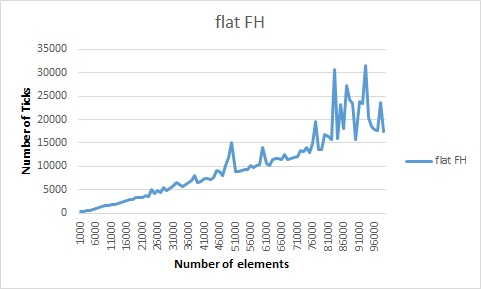
\includegraphics[width=15cm, height=9cm]{Flat FH pop.jpg}
        \centering
    \end{figure}
    \begin{figure}[h]
        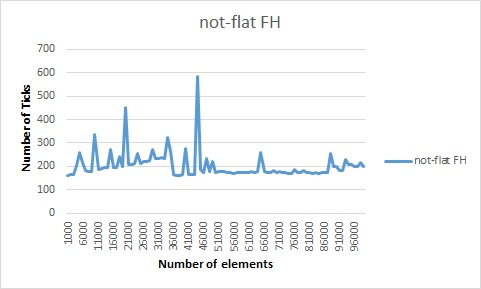
\includegraphics[width=15cm, height=9cm]{non-Flat FH pop.jpg}
        \centering
    \end{figure}
    \begin{figure}[h]
        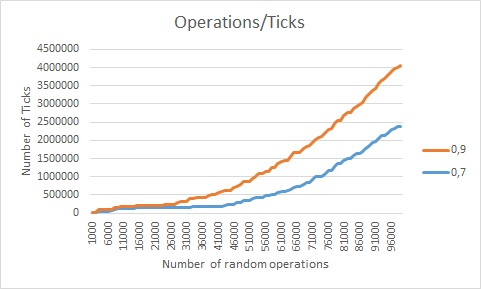
\includegraphics[width=15cm, height=9cm]{summary time of several operations.jpg}
        \centering
    \end{figure}
\end{document}
	